        %%******************************************%%
        %%                                          %%
        %%        Modello di tesi di laurea         %%
        %%            di Andrea Giraldin            %%
        %%                                          %%
        %%             2 novembre 2012              %%
        %%                                          %%
        %%******************************************%%


% I seguenti commenti speciali impostano:
% 1. 
% 2. PDFLaTeX come motore di composizione;
% 3. tesi.tex come documento principale;
% 4. il controllo ortografico italiano per l'editor.

% !TEX encoding = UTF-8
% !TEX TS-program = pdflatex
% !TEX root = tesi.tex
% !TEX spellcheck = it-IT

% PDF/A filecontents
\RequirePackage{filecontents}
\begin{filecontents*}{\jobname.xmpdata}
  \Title{Document's title}
  \Author{Author's name}
  \Language{it-IT}
  \Subject{The abstract, or short description.}
  \Keywords{keyword1\sep keyword2\sep keyword3}
\end{filecontents*}

\documentclass[10pt,                    % corpo del font principale
               a4paper,                 % carta A4
               twoside,                 % impagina per fronte-retro
               openright,               % inizio capitoli a destra
               english,                 
               italian,                 
               ]{book}    

%**************************************************************
% Importazione package
%************************************************************** 

\PassOptionsToPackage{dvipsnames}{xcolor} % colori PDF/A

\usepackage{colorprofiles}

\usepackage[a-2b,mathxmp]{pdfx}[2018/12/22]
                                        % configurazione PDF/A
                                        % validare in https://www.pdf-online.com/osa/validate.aspx

%\usepackage{amsmath,amssymb,amsthm}    % matematica

\usepackage[T1]{fontenc}                % codifica dei font:
                                        % NOTA BENE! richiede una distribuzione *completa* di LaTeX

\usepackage[utf8]{inputenc}             % codifica di input; anche [latin1] va bene
                                        % NOTA BENE! va accordata con le preferenze dell'editor

\usepackage[english, italian]{babel}    % per scrivere in italiano e in inglese;
                                        % l'ultima lingua (l'italiano) risulta predefinita

\usepackage{bookmark}                   % segnalibri

\usepackage{caption}                    % didascalie

\usepackage{chngpage,calc}              % centra il frontespizio

\usepackage{csquotes}                   % gestisce automaticamente i caratteri (")

\usepackage{emptypage}                  % pagine vuote senza testatina e piede di pagina

\usepackage{epigraph}			% per epigrafi

\usepackage{eurosym}                    % simbolo dell'euro

\usepackage{indentfirst}               % rientra il primo paragrafo di ogni sezione

\usepackage{graphicx}                   % immagini

\usepackage{hyperref}                   % collegamenti ipertestuali

\usepackage[binding=5mm]{layaureo}      % margini ottimizzati per l'A4; rilegatura di 5 mm

\usepackage{listings}                   % codici

\usepackage{microtype}                  % microtipografia

\usepackage{mparhack,fixltx2e,relsize}  % finezze tipografiche

\usepackage{nameref}                    % visualizza nome dei riferimenti                                      
\usepackage[font=small]{quoting}        % citazioni

\usepackage{subfig}                     % sottofigure, sottotabelle

\usepackage[italian]{varioref}          % riferimenti completi della pagina

\usepackage{booktabs}                   % tabelle                                       
\usepackage{tabularx}                   % tabelle di larghezza prefissata                                    
\usepackage{longtable}                  % tabelle su più pagine                                        
\usepackage{ltxtable}                   % tabelle su più pagine e adattabili in larghezza

\usepackage[toc, acronym]{glossaries}   % glossario
                                        % per includerlo nel documento bisogna:
                                        % 1. compilare una prima volta tesi.tex;
                                        % 2. eseguire: makeindex -s tesi.ist -t tesi.glg -o tesi.gls tesi.glo
                                        % 3. eseguire: makeindex -s tesi.ist -t tesi.alg -o tesi.acr tesi.acn
                                        % 4. compilare due volte tesi.tex.

\usepackage[backend=biber,style=verbose-ibid,hyperref,backref]{biblatex}
                                        % eccellente pacchetto per la bibliografia; 
                                        % produce uno stile di citazione autore-anno; 
                                        % lo stile "numeric-comp" produce riferimenti numerici
                                        % per includerlo nel documento bisogna:
                                        % 1. compilare una prima volta tesi.tex;
                                        % 2. eseguire: biber tesi
                                        % 3. compilare ancora tesi.tex.

%**************************************************************
% file contenente le impostazioni della tesi
%**************************************************************

%**************************************************************
% Frontespizio
%**************************************************************

% Autore
\newcommand{\myName}{Riccardo Tassetto}                                    
\newcommand{\myTitle}{Sviluppo software per la gestione di offerte di fornitura e richieste di acquisto di beni materiali}

% Tipo di tesi                   
\newcommand{\myDegree}{Tesi di laurea}

% Università             
\newcommand{\myUni}{Università degli Studi di Padova}

% Facoltà       
\newcommand{\myFaculty}{Corso di Laurea in Informatica}

% Dipartimento
\newcommand{\myDepartment}{Dipartimento di Matematica "Tullio Levi-Civita"}

% Titolo del relatore
\newcommand{\profTitle}{Prof.}

% Relatore
\newcommand{\myProf}{Tullio Vardanega}

% Luogo
\newcommand{\myLocation}{Padova}

% Anno accademico
\newcommand{\myAA}{2019-2020}

% Data discussione
\newcommand{\myTime}{Dicembre 2020}


%**************************************************************
% Impostazioni di impaginazione
% see: http://wwwcdf.pd.infn.it/AppuntiLinux/a2547.htm
%**************************************************************

\setlength{\parindent}{14pt}   % larghezza rientro della prima riga
\setlength{\parskip}{0pt}   % distanza tra i paragrafi


%**************************************************************
% Impostazioni di biblatex
%**************************************************************
\bibliography{bibliografia} % database di biblatex 

\defbibheading{bibliography} {
    \cleardoublepage
    \phantomsection 
    \addcontentsline{toc}{chapter}{\bibname}
    \chapter*{\bibname\markboth{\bibname}{\bibname}}
}

\setlength\bibitemsep{1.5\itemsep} % spazio tra entry

\DeclareBibliographyCategory{opere}
\DeclareBibliographyCategory{web}

\addtocategory{opere}{womak:lean-thinking}
\addtocategory{web}{site:agile-manifesto}

\defbibheading{opere}{\section*{Riferimenti bibliografici}}
\defbibheading{web}{\section*{Siti Web consultati}}


%**************************************************************
% Impostazioni di caption
%**************************************************************
\captionsetup{
    tableposition=top,
    figureposition=bottom,
    font=small,
    format=hang,
    labelfont=bf
}

%**************************************************************
% Impostazioni di glossaries
%**************************************************************

%**************************************************************
% Acronimi
%**************************************************************
\renewcommand{\acronymname}{Acronimi e abbreviazioni}

\newacronym[description={\glslink{apig}{Application Program Interface}}]
    {api}{API}{Application Program Interface}

\newacronym[description={\glslink{umlg}{Unified Modeling Language}}]
    {uml}{UML}{Unified Modeling Language}
    
\newacronym[description={\glslink{bi}{Business Intelligence}}]
    {bi}{BI}{Business Intelligence}
    
\newacronym[description={\glslink{ict}{Information and Communications Technology}}]
	{ict}{ICT}{Information and Communications Technology}

%**************************************************************
% Glossario
%**************************************************************
\renewcommand{\glossaryname}{Glossario}

\newglossaryentry{apig}
{
    name=\glslink{api}{API},
    text=Application Program Interface,
    sort=api,
    description={in informatica con il termine \emph{Application Programming Interface API} (ing. interfaccia di programmazione di un'applicazione) si indica ogni insieme di procedure disponibili al programmatore, di solito raggruppate a formare un set di strumenti specifici per l'espletamento di un determinato compito all'interno di un certo programma. La finalità è ottenere un'astrazione, di solito tra l'hardware e il programmatore o tra software a basso e quello ad alto livello semplificando così il lavoro di programmazione}
}

\newglossaryentry{ictg}
{
	name=\glslink{ict}{ICT},
	text=Information and Communications Technology,
	sort=ict,
	description={le tecnologie dell'informazione e della comunicazione, acronimo ICT, sono l'insieme dei metodi e delle tecniche utilizzate nella trasmissione, ricezione ed elaborazione di dati e informazioni}
}

\newglossaryentry{big}
{
	name=\glslink{bi}{Business Intelligence},
	text=Business Intelligence,
	sort=bi,
	description={Con la locuzione \textit{Business Intelligence} (\textit{BI}) ci si può solitamente riferire a tre elementi, quali: un insieme di processi aziendali per raccogliere dati ed analizzare informazioni strategiche; la tecnologia utilizzata per realizzare questi processi; le informazioni ottenute come risultato di questi processi}
}
 % database di termini
\makeglossaries


%**************************************************************
% Impostazioni di graphicx
%**************************************************************
\graphicspath{{immagini/}} % cartella dove sono riposte le immagini


%**************************************************************
% Impostazioni di hyperref
%**************************************************************
\hypersetup{
    %hyperfootnotes=false,
    %pdfpagelabels,
    %draft,	% = elimina tutti i link (utile per stampe in bianco e nero)
    colorlinks=true,
    linktocpage=true,
    pdfstartpage=1,
    pdfstartview=,
    % decommenta la riga seguente per avere link in nero (per esempio per la stampa in bianco e nero)
    %colorlinks=false, linktocpage=false, pdfborder={0 0 0}, pdfstartpage=1, pdfstartview=FitV,
    breaklinks=true,
    pdfpagemode=UseNone,
    pageanchor=true,
    pdfpagemode=UseOutlines,
    plainpages=false,
    bookmarksnumbered,
    bookmarksopen=true,
    bookmarksopenlevel=1,
    hypertexnames=true,
    pdfhighlight=/O,
    %nesting=true,
    %frenchlinks,
    urlcolor=webbrown,
    linkcolor=RoyalBlue,
    citecolor=webgreen,
    %pagecolor=RoyalBlue,
    %urlcolor=Black, linkcolor=Black, citecolor=Black, %pagecolor=Black,
    pdftitle={\myTitle},
    pdfauthor={\textcopyright\ \myName, \myUni, \myFaculty},
    pdfsubject={},
    pdfkeywords={},
    pdfcreator={pdfLaTeX},
    pdfproducer={LaTeX}
}

%**************************************************************
% Impostazioni di itemize
%**************************************************************
\renewcommand{\labelitemi}{$\ast$}

%\renewcommand{\labelitemi}{$\bullet$}
%\renewcommand{\labelitemii}{$\cdot$}
%\renewcommand{\labelitemiii}{$\diamond$}
%\renewcommand{\labelitemiv}{$\ast$}


%**************************************************************
% Impostazioni di listings
%**************************************************************
\lstset{
    language=[LaTeX]Tex,%C++,
    keywordstyle=\color{RoyalBlue}, %\bfseries,
    basicstyle=\small\ttfamily,
    %identifierstyle=\color{NavyBlue},
    commentstyle=\color{Green}\ttfamily,
    stringstyle=\rmfamily,
    numbers=none, %left,%
    numberstyle=\scriptsize, %\tiny
    stepnumber=5,
    numbersep=8pt,
    showstringspaces=false,
    breaklines=true,
    frameround=ftff,
    frame=single
} 


%**************************************************************
% Impostazioni di xcolor
%**************************************************************
\definecolor{webgreen}{rgb}{0,.5,0}
\definecolor{webbrown}{rgb}{.6,0,0}


%**************************************************************
% Altro
%**************************************************************

\newcommand{\omissis}{[\dots\negthinspace]} % produce [...]

% eccezioni all'algoritmo di sillabazione
\hyphenation
{
    ma-cro-istru-zio-ne
    gi-ral-din
}

\newcommand{\sectionname}{sezione}
\addto\captionsitalian{\renewcommand{\figurename}{Figura}
                       \renewcommand{\tablename}{Tabella}}

\newcommand{\glsfirstoccur}{\ap{{[g]}}}

\newcommand{\intro}[1]{\emph{\textsf{#1}}}

%**************************************************************
% Environment per ``rischi''
%**************************************************************
\newcounter{riskcounter}                % define a counter
\setcounter{riskcounter}{0}             % set the counter to some initial value

%%%% Parameters
% #1: Title
\newenvironment{risk}[1]{
    \refstepcounter{riskcounter}        % increment counter
    \par \noindent                      % start new paragraph
    \textbf{\arabic{riskcounter}. #1}   % display the title before the 
                                        % content of the environment is displayed 
}{
    \par\medskip
}

\newcommand{\riskname}{Rischio}

\newcommand{\riskdescription}[1]{\textbf{\\Descrizione:} #1.}

\newcommand{\risksolution}[1]{\textbf{\\Soluzione:} #1.}

%**************************************************************
% Environment per ``use case''
%**************************************************************
\newcounter{usecasecounter}             % define a counter
\setcounter{usecasecounter}{0}          % set the counter to some initial value

%%%% Parameters
% #1: ID
% #2: Nome
\newenvironment{usecase}[2]{
    \renewcommand{\theusecasecounter}{\usecasename #1}  % this is where the display of 
                                                        % the counter is overwritten/modified
    \refstepcounter{usecasecounter}             % increment counter
    \vspace{10pt}
    \par \noindent                              % start new paragraph
    {\large \textbf{\usecasename #1: #2}}       % display the title before the 
                                                % content of the environment is displayed 
    \medskip
}{
    \medskip
}

\newcommand{\usecasename}{UC}

\newcommand{\usecaseactors}[1]{\textbf{\\Attori Principali:} #1. \vspace{4pt}}
\newcommand{\usecasepre}[1]{\textbf{\\Precondizioni:} #1. \vspace{4pt}}
\newcommand{\usecasedesc}[1]{\textbf{\\Descrizione:} #1. \vspace{4pt}}
\newcommand{\usecasepost}[1]{\textbf{\\Postcondizioni:} #1. \vspace{4pt}}
\newcommand{\usecasealt}[1]{\textbf{\\Scenario Alternativo:} #1. \vspace{4pt}}

%**************************************************************
% Environment per ``namespace description''
%**************************************************************

\newenvironment{namespacedesc}{
    \vspace{10pt}
    \par \noindent                              % start new paragraph
    \begin{description} 
}{
    \end{description}
    \medskip
}

\newcommand{\classdesc}[2]{\item[\textbf{#1:}] #2}
                     % file con le impostazioni personali

\begin{document}
%**************************************************************
% Materiale iniziale
%**************************************************************
\frontmatter
% !TEX encoding = UTF-8
% !TEX TS-program = pdflatex
% !TEX root = ../tesi.tex

%**************************************************************
% Frontespizio 
%**************************************************************
\begin{titlepage}

\begin{center}

\begin{LARGE}
\textbf{\myUni}\\
\end{LARGE}

\vspace{10pt}

\begin{Large}
\textsc{\myDepartment}\\
\end{Large}

\vspace{10pt}

\begin{large}
\textsc{\myFaculty}\\
\end{large}

\vspace{30pt}
\begin{figure}[htbp]
\begin{center}
\includegraphics[height=6cm]{logo-unipd}
\end{center}
\end{figure}
\vspace{30pt} 

\begin{Large}
\begin{center}
\textbf{\myTitle}\\
\end{center}
\end{Large}

\vspace{10pt} 

\begin{large}
\textsl{\myDegree}\\
\end{large}

\vspace{35pt} 

\begin{large}
\begin{flushleft}
\textit{Relatore}\\ 
\vspace{5pt} 
\profTitle \myProf
\end{flushleft}

\vspace{0pt} 

\begin{flushright}
\textit{Laureando}\\ 
\vspace{5pt} 
\myName
\end{flushright}
\end{large}

\vspace{35pt}

\line(1, 0){338} \\
\begin{normalsize}
\textsc{Anno Accademico \myAA}
\end{normalsize}

\end{center}
\end{titlepage} 
\input{inizio-fine/colophon}
%\input{inizio-fine/dedica}
% !TEX encoding = UTF-8
% !TEX TS-program = pdflatex
% !TEX root = ../tesi.tex

%**************************************************************
% Sommario
%**************************************************************
\cleardoublepage
\phantomsection
\pdfbookmark{Sommario}{Sommario}
\begingroup
\let\clearpage\relax
\let\cleardoublepage\relax
\let\cleardoublepage\relax

\chapter*{Sommario}

Il presente documento descrive il \textit{stage} da me svolto presso l'azienda San Marco Group S.p.A. nella sede di Marcon (VE), nel periodo che va dal 03-08-2020 al 06-11-2020. L'esperienza di \textit{stage} ha avuto una durata complessiva di 320 ore ed è stata supervisionata e coordinata sia dal mio tutor aziendale, Mauro Vecchiato, che dal mio relatore presso l'ateneo, prof. Tullio Vardanega.\\
Lo scopo principale di questo progetto di \textit{stage} consisteva nello sviluppo di un sistema di gestione di offerte di fornitura, dedicate a beni materiali e servizi.\\
In particolare, una volta analizzato il processo aziendale ed essermi interfacciato con gli utenti coinvolti per identificare la soluzione progettuale più adatta, ho progettato un'interfaccia del gestionale utilizzata dagli utenti interni all'azienda e ho sviluppato un'applicazione \textit{web} utilizzabile dai fornitori per rispondere alle richieste di offerta.\\
Ho suddiviso il presente documento in 4 capitoli:
\begin{itemize}
	\item \textbf{Capitolo 1}: presentazione del contesto aziendale, processi interni e propensione all'innovazione;
	\item \textbf{Capitolo 2}: presentazione dell'offerta di \textit{stage} e motivazioni della scelta effettuata; 
	\item \textbf{Capitolo 3}: presentazione dettagliata del progetto, con approfondimento delle sue fasi, delle tecnologie utilizzate e delle soluzioni attuate per realizzarlo;
	\item \textbf{Capitolo 4}: resoconto del lavoro svolto con una valutazione personale sugli obiettivi raggiunti, le difficoltà incontrate e le conoscenze personali e professionali acquisite.
\end{itemize}
Per la redazione del documento ho adottato le seguenti norme tipografiche:
\begin{itemize}
\item ho scritto in corsivo i termini in lingua diversa dall'italiano;
\item ho scritto in corsivo e marcato con una G maiuscola a pedice i termini del Glossario presenti nel testo alla loro prima occorrenza.
\end{itemize}

\vfill
%
%\selectlanguage{english}
%\pdfbookmark{Abstract}{Abstract}
%\chapter*{Abstract}
%
%\selectlanguage{italian}

\endgroup			

\vfill


%% !TEX encoding = UTF-8
% !TEX TS-program = pdflatex
% !TEX root = ../tesi.tex

%**************************************************************
% Ringraziamenti
%**************************************************************
\cleardoublepage
\phantomsection
\pdfbookmark{Ringraziamenti}{ringraziamenti}

%**************************************************************
%\begin{flushright}{
%	\slshape    
%	``Life is really simple, but we insist on making it complicated''} \\ 
%	\medskip
%    --- Confucius
%\end{flushright}
%**************************************************************

%\bigskip

\begingroup
\let\clearpage\relax
\let\cleardoublepage\relax
\let\cleardoublepage\relax

\chapter*{Ringraziamenti}

\noindent \textit{Innanzitutto, vorrei esprimere la mia gratitudine al \profTitle \myProf, relatore della mia tesi, per l'aiuto e il sostegno fornitomi durante la stesura del lavoro.}\\

\noindent \textit{Desidero ringraziare con affetto i miei genitori per il sostegno, il grande aiuto e per essermi stati vicini in ogni momento durante gli anni di studio.}\\

%\noindent \textit{Ho desiderio di ringraziare poi i miei amici per tutti i %bellissimi anni passati insieme e le mille avventure vissute.}\\
%\bigskip

\noindent\textit{\myLocation, \myTime}
\hfill \myName

\endgroup


\input{inizio-fine/indici}
\cleardoublepage

%**************************************************************
% Materiale principale
%**************************************************************
\mainmatter
% !TEX encoding = UTF-8
% !TEX TS-program = pdflatex
% !TEX root = ../tesi.tex

%**************************************************************
\chapter{Analisi del contesto aziendale}
\label{cap:introduzione}
%**************************************************************

Introduzione al contesto applicativo.\\

\noindent Esempio di utilizzo di un termine nel glossario \\
\gls{api}. \\

\noindent Esempio di citazione in linea \\
\cite{site:agile-manifesto}. \\

\noindent Esempio di citazione nel pie' di pagina \\
citazione\footcite{womak:lean-thinking} \\

%**************************************************************
\section{L’azienda San Marco Group}

San Marco Group è un gruppo aziendale leader in Italia nella produzione di pitture e vernici per l’edilizia professionale. Il Gruppo con sede principale a Marcon (VE) oggi conta 8 siti produttivi ed è proprietario di 7 diversi brand, ha un fatturato pari a 80 milioni di euro e una rete distributiva che tocca oltre 100 Paesi.

%**************************************************************
\section{Organizzazione del lavoro}

Introduzione all'idea dello stage.

%**************************************************************
\section{Tecnologie utilizzate}

Descrizione delle tecnologie utilizzate.

%**************************************************************
\section{Organizzazione del testo}

\begin{description}
    \item[{\hyperref[cap:processi-metodologie]{Il secondo capitolo}}] descrive ...
    
    \item[{\hyperref[cap:descrizione-stage]{Il terzo capitolo}}] approfondisce ...
    
    \item[{\hyperref[cap:analisi-requisiti]{Il quarto capitolo}}] approfondisce ...
    
    \item[{\hyperref[cap:progettazione-codifica]{Il quinto capitolo}}] approfondisce ...
    
    \item[{\hyperref[cap:verifica-validazione]{Il sesto capitolo}}] approfondisce ...
    
    \item[{\hyperref[cap:conclusioni]{Nel settimo capitolo}}] descrive ...
\end{description}

Riguardo la stesura del testo, relativamente al documento sono state adottate le seguenti convenzioni tipografiche:
\begin{itemize}
	\item gli acronimi, le abbreviazioni e i termini ambigui o di uso non comune menzionati vengono definiti nel glossario, situato alla fine del presente documento;
	\item per la prima occorrenza dei termini riportati nel glossario viene utilizzata la seguente nomenclatura: \emph{parola}\glsfirstoccur;
	\item i termini in lingua straniera o facenti parti del gergo tecnico sono evidenziati con il carattere \emph{corsivo}.
\end{itemize}             % Introduzione azienda
% !TEX encoding = UTF-8
% !TEX TS-program = pdflatex
% !TEX root = ../tesi.tex

%**************************************************************
\chapter{Progetto di stage}
\label{cap:progetto-di-stage}
%**************************************************************


%**************************************************************
\section{Lo stage per San Marco Group}

Il concetto di stage formativo è molto importante per l'azienda San Marco Group. 
In primo luogo, viene considerata la sperimentazione di nuove tecnologie ed il loro confronto con quelle utilizzate quotidianamente. Per poterlo fare attualmente il personale presente dovrebbe smettere di svolgere le proprie attività, per questo motivo uno stagista universitario diventa una risorsa indispensabile, permettendo quindi all'azienda di sperimentare senza che vengano bloccate le normali mansioni.
Ci sono diverse realtà all'interno dell'azienda che possono considerarsi formative per uno studente e che attuano costantemente questa collaborazione:
\begin{itemize}
	\item \textbf{l'ufficio Risorse Umane}, dove studenti del settore giuridico o umanistico possono crescere trovandosi in un'azienda con un grande gruppo eterogeneo di membri; 
	\item \textbf{l'ufficio Marketing}, molto sviluppato nell'azienda che dà spazio a figure che hanno intrapreso studi in ambito grafico o orientati alle comunicazioni e al \textit{marketing web};
	\item \textbf{il laboratorio di Ricerca e Sviluppo}, la sezione, presente nella sede di Marcon, affianca studenti del settore chimico ad un gruppo di chimici \textit{senior} che svolge attività di studio e ricerca su pitture decorative e decorativi per pavimenti, prodotti per le facciate, rivestimenti e sistemi termoisolanti; 
	\item \textbf{i Back office}, che comprendono l'ufficio Acquisti e l'ufficio Commerciale, dove studenti nel settore economico e commerciale hanno modo di confrontarsi con una realtà molto sviluppata e affermata nel territorio.
\end{itemize}
In secondo luogo, l'instaurazione del rapporto con l'Università di Padova è dato dalla possibilità di inserimento nell'azienda di risorse derivanti dal mondo accademico che, con una nuova prospettiva data dalle conoscenze apprese e messe in pratica nel corso di studio, possono portare idee creative e innovative, dalle quali può trarre beneficio anche il personale aziendale.

%**************************************************************
\section{Contesto attuale}

Attualmente l'azienda è nel vivo di un progetto di cambio gestionale, motivato principalmente da:
\begin{itemize}
	\item la fine del supporto da parte di \textit{Microsoft}, sul gestionale attualmente adottato (\textit{Microsoft Dynamics Ax 2009}) fissato per il 12 ottobre 2021;
	\item insoddisfazione da parte della direzione sul prodotto.
\end{itemize}
Nonostante ci fosse la possibilità di continuare ad utilizzare la versione 2009 anche oltre alla fine del supporto, affidandosi ad un partner terzo per la manutenzione e le implementazioni dei vari adeguamenti necessari a soddisfare periodicamente le regole stabilite nel contesto fiscale, tale decisione è stata ritenuta troppo rischiosa perché in caso di inadempienze del partner scelto, ci sarebbero potute essere conseguenze importanti per l'azienda, come ad esempio l'impossibilità di adempiere agli obblighi fiscali.
Si è deciso quindi di effettuare l'analisi di tutti i processi aziendali così da individuarne le criticità: in questo modo il cambio di \textit{software} non avrebbe solamente soddisfatto le necessità ma anche portato un miglioramento. In seguito all'analisi supportata da un'azienda di consulenza, è iniziata la \textit{software selection}.

\vspace{10pt}
\begin{figure}[htbp]
	\begin{center}
		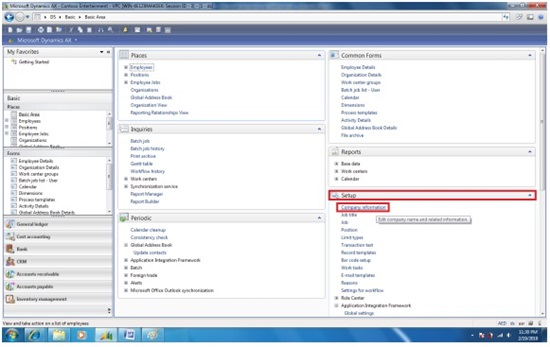
\includegraphics[height=8cm]{ax-2009}
		\caption{Interfaccia utente \textit{Microsoft Dynamics Ax 2009}. \newline \textbf{Fonte: }\url{https://community.dynamics.com/}}
	\end{center}
\end{figure}
\vspace{10pt}

Tra i vari \textit{software} gestionali presenti sul mercato, è stato preso in considerazione \textit{Microsoft Dynamics 365}. La nuova versione dell'\textit{ERP} di \textit{Microsoft} differisce in maniera sostanziale da quella attualmente utilizzata, principalmente per quanto riguarda:
\begin{itemize}
	\item la re-ingegnerizzazione della base di dati, che richiederebbe una reimpostazione radicale della base di dati attuale;
	\item la dismissione del modello di sviluppo a \textit{layer}, che consiste nell'utilizzo di una gerarchia di livelli nei quali vengono implementati i metodi degli elementi applicativi presenti nel gestionale. Quando viene eseguito un metodo di un qualsiasi elemento applicativo, il sistema parte dal \textit{layer} più esterno per verificare ed eseguire, se disponibile, un'implementazione del metodo per quell'elemento, altrimenti si sposta sul \textit{layer} più interno per ripetere l'operazione fino ad arrivare al \textit{layer} di sistema.In questo modo è possibile personalizzare facilmente le varie funzionalità presenti, attività che con la nuova versione richiederebbero un processo più impegnativo.
\end{itemize}
L'adozione di \textit{Microsoft Dynamics 365} sarebbe stata troppo impegnativa dal punto di vista tecnico sia nel breve che nel lungo termine, per questo motivo è stato scartato.
Alla fine della valutazione la scelta è ricaduta su Sage X3, per la sua adattabilità e perché rispecchia maggiormente le necessità aziendali; è perciò iniziata la fase di implementazione del nuovo \textit{software} attraverso:

\begin{itemize}
	\item sviluppi per adeguamento delle funzionalità del nuovo gestionale agli standard aziendali;
	\item migrazione dei dati;
	\item formazione degli utenti finali.
\end{itemize}


\vspace{10pt}
\begin{figure}[htbp]
	\begin{center}
		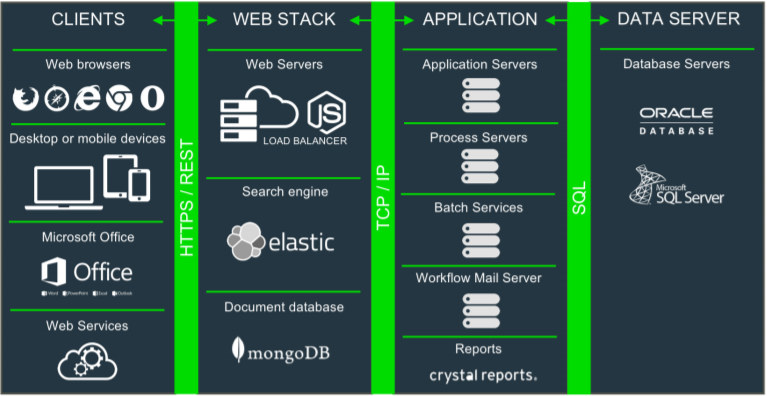
\includegraphics[height=7cm]{sage-x3}
		\caption{Architettura di sistema di Sage X3. \newline \textbf{Fonte:}\url{https://partnerportal.sagex3.com/}}
	\end{center}
\end{figure}
\vspace{30pt}


%**************************************************************
\section{Proposta di stage}

Lo scopo dello stage consisteva nello sviluppo \textit{software} di un sistema di gestione di offerte di fornitura, dedicate a beni materiali e servizi. Dopo l'analisi del processo, dovevo sviluppare un'applicazione \textit{web} che permettesse agli utenti interni la gestione delle richieste e ai fornitori designati di rispondere con delle proposte di offerta.
L'applicazione da sviluppare doveva avere le seguenti caratteristiche:
\begin{itemize}
	\item interfacciarsi con il database del gestionale tramite \textit{web service};
	\item la sezione destinata alle richieste di servizio di trasporto doveva rispettare il layout del modulo cartaceo utilizzato;
\end{itemize}
Dovevo produrre un \textit{report} con il dettaglio della richiesta e in base al tempo disponibile, riuscire a fornire delle statistiche sulla base dei dati utilizzati, utili all'analisi di \textit{BI}, in ottica di miglioramento del processo aziendale.


\subsection{Prodotti attesi}
L'attività di stage prevedeva la produzione dei seguenti oggetti, documenti e \textit{software}:
\begin{itemize}
	\item relazione sul processo aziendale coinvolto;
	\item relazione sulla progettazione architetturale;
	\item codice sorgente dell'applicazione \textit{web};
	\item manuale e documentazione riguardante la struttura dell'applicazione \textit{web} per
	manutenzione ed eventuali integrazioni;
	\item \textit{report} di dettaglio dell'offerta;
	\item \textit{report} con statistiche utili all'analisi di \textit{BI}.
\end{itemize}


\subsection{Priorità e obiettivi dello stage}
Per identificare gli obiettivi ed il loro livello di priorità, ho associato a ciascuno di essi un codice nel formato sottostante:
\\
\begin{center}
	\textit{<obiettivo.[sotto-obiettivo]-tipologia>. }
\end{center}
Il significato del codice è il seguente:
\begin{itemize}
\item \textbf{obiettivo}, indica il numero univoco dell'obiettivo;
\item \textbf{sotto-obiettivo}, è il numero univoco del sotto-obiettivo, ed è opzionale, essendo riportato solo nel caso in cui l'obiettivo sia suddiviso in sotto-obiettivi;
\item \textbf{tipologia}, indica il livello di priorità assegnato all'obiettivo.
\end{itemize}
La tipologia determina l'importanza di realizzare tale obiettivo, ed è scelta tra le seguenti:
\begin{itemize}
	\item \textbf{OB}, indica un obiettivo obbligatorio, il cui raggiungimento è necessario;
	\item \textbf{DE}, indica un obiettivo desiderabile, il cui raggiungimento è importante e dal riconoscibile valore aggiunto, ma non necessario.
\end{itemize}

\begin{center}
	\begin{longtable}{ | c| c |}
		\caption{Tabella riassuntiva degli gli obiettivi dello stage.}\\
		\hline
		\textbf{Obiettivo} & \textbf{Descrizione}\\
		\hline
		1-OB & Comprensione del problema\\
		\hline
		2-OB & Comprensione delle tecnologie di \textit{backend}\\
		\hline
		2.1-OB & Comprensione di \textit{Sage X3}\\
		\hline
		2.2-OB & Comprensione del database \textit{SQL Server}\\
		\hline
		2.3-OB & Comprensione della tecnologia dei \textit{web service}\\
		\hline
		3-OB & Comprensione delle tecnologie di \textit{frontend}\\
		\hline
		3.1-OB & Comprensione di \textit{Javascript}\\
		\hline
		3.2-OB & Comprensione di \textit{JQuery}\\
		\hline
		4-OB & Sviluppo dell'applicazione \textit{web}\\
		\hline
		5-OB & Sviluppo del \textit{report} per tracciamento caratteristiche offerta\\
		\hline
		6-OB & Validazione del prodotto\\
		\hline
		7-DE & Sviluppo del \textit{report} per statistiche miglioramento \textit{BI}\\
		\hline
	\end{longtable}
\end{center}


\subsection{Vincoli}
\subsubsection{Vincoli temporali e organizzativi}
Il progetto di stage ha avuto una durata di 320 ore, distribuite nell'arco di tre mesi, con settimane lavorative di 25 ore ciascuna.
In accordo con il relatore e il tutor aziendale, lo stage è stato svolto prevalentemente in modalità \textit{smart working}.
Per poter informare il mio relatore  dei progressi, ogni 5 giorni lavorativi dovevo provvedere a inviare un resoconto dello stato di avanzamento rispetto alle attese del piano di lavoro e ad eventuali deviazioni da esso.\\Invece, con il tutor aziendale, ho previsto almeno un incontro a settimana in remoto o fisicamente in azienda per discutere del progresso e di eventuali cambiamenti da apportare al progetto.
\subsubsection{Vincoli tecnologici}
Lo sviluppo del progetto prevedeva alcuni vincoli imposti dall'azienda.
In primo luogo l'utilizzo della tecnologia \textit{SOAP}, \textit{Simple Object Access Protocol}, per i \textit{web service} che permettevano l'interfacciamento tra l'applicazione \textit{web} e il gestionale.
In secondo luogo, l'utilizzo dello strumento per la produzione di stampe di dati \textit{Crystal Reports} per produrre il \textit{report} di dettaglio della richiesta d'offerta e il \textit{report} con le statistiche utili all'analisi della \textit{BI}.


\subsection{Pianificazione}

Il Piano di Lavoro, redatto insieme al tutor aziendale, prevedeva inizialmente 4 fasi, ognuna delle quali della durata di 3 settimane lavorative:
\begin{itemize}
	\item studio del processo aziendale e formazione sulle tecnologie coinvolte nello sviluppo dell'applicazione \textit{web} e dell'interfacciamento con il gestionale;
	\item progettazione della soluzione e configurazione dell'ambiente di sviluppo;
	\item realizzazione dell'applicazione \textit{web} e fase di \textit{testing};
	\item formazione sul \textit{software} per la produzione di stampe e sviluppo dei \textit{report};
\end{itemize}
L'ultima settimana di stage prevedeva la verifica e validazione finale.
Di seguito un dettaglio delle fasi appena descritte:

\begin{center}
	\begin{longtable}{|c|c|}
		\caption{Dettaglio pianificazione del progetto di stage.}\\		
		\hline
		\textbf{Ore} & \textbf{Attività}\\
		\hline
		40 & Formazione sulle tecnologie\\
		\hline
		35 & Analisi del problema\\
		\hline
		25 & Stesura documentazione relativa ad analisi e progettazione\\
		\hline
		55 & Progettazione della soluzione\\
		\hline
		15 & Configurazione dell'ambiente di sviluppo\\
		\hline
		60 & Sviluppo dell'applicazione \textit{web}\\
		\hline
		20 & \textit{Test} sull'applicazione \textit{web}\\
		\hline
		25 & \textit{Test} sui \textit{web service}\\
		\hline
		25 & Formazione su strumento e produzione \textit{report}\\
		\hline
		5 & Stesura documentazione finale\\
		\hline
		15 & Verifica e validazione finale\\
		\hline
	\end{longtable}
\end{center}


%**************************************************************
\section{Analisi preventiva dei rischi}
Nella fase iniziale di analisi ho individuato alcuni possibili rischi in cui poter incorrere.\\
Successivamente, ho provveduto ad elaborare delle possibili soluzioni per far loro fronte.
\\
\begin{risk}{Tecnologie e \textit{framework} sconosciuti}
	\riskdescription{Durante lo svolgimento dello stage è previsto l'utilizzo di tecnologie a me ancora sconosciute}
	\risksolution{Nella fase di pianificazione iniziale ho programmato un periodo di auto-formazione sulle tecnologie e sui \textit{framework} da utilizzare}	
\end{risk}
\begin{risk}{Incomprensioni sul processo aziendale}
	\riskdescription{A causa dei vari enti coinvolti nella fase di analisi e del gran numero di attività svolte attualmente extra sistema (utilizzo di moduli cartacei, contatti telefonici direttamente coi fornitori, ecc.), è possibile non riesca a delineare e comprendere pienamente il processo aziendale interessato}
	\risksolution{In accordo con il \textit{tutor} aziendale, sono stati individuati dei \textit{key users}, uno per ogni ufficio coinvolto, che si rendono disponibili ad offrire maggior dettaglio sulle fasi che interessano la loro attività}	
\end{risk}
\begin{risk}{Scelte non ottimali}
	\riskdescription{A causa dell'inesperienza è possibile che io non comprenda le attività da svolgere o faccia scelte non adeguate alle aspettative.}
	\risksolution{Tutte le scelte progettuali fondamentali saranno discusse e supervisionate dal \textit{tutor} aziendale}	
\end{risk}

%**************************************************************
\section{Motivazione della scelta}

\subsection{Motivazioni personali}

Una delle principali aspettative che mi hanno portato a scegliere questa proposta di stage curriculare, era il contesto di inserimento: volevo capire come una grande azienda, il cui settore di impiego non è strettamente legato a quello informatico, si approccia alle nuove tecnologie e si appoggia all'informatica per il suo business. 
\\
Riuscire ad avere una visione d'insieme per capire quali attività vengono svolte per supportare un'azienda, non solo del contesto dello sviluppo \textit{software} ma anche nell'ausilio di altri processi.
\\
Inoltre, l'opportunità offertami dall'azienda non si sarebbe fermata al semplice stage curricolare o viceversa all'assunzione per la sola occupazione lavorativa, ma quella che mi è stata proposta era contemporaneamente la possibilità di supporto nel mio percorso di studi fornendomi un impiego retribuito, a riprova di una \textit{vision} contemporanea che vede negli stagisti non uno svantaggio, ma una risorsa che porta nuova linfa all'interno di un mondo lavorativo consolidato.
\\
A conclusione dello stage mi attirava la possibilità di continuare a seguire le attività successive allo sviluppo del prodotto, come la formazione degli utenti, e vedere i risultati del mio lavoro nel lungo termine.

\subsection{Motivazioni professionali}

La mia scelta di stage è ricaduta su questa azienda perché rispetto alle altre con cui ho avuto contatti grazie all'evento di incontro \textit{StageIt} in cui le principali aziende del territorio propongono i loro \textit{stage} formativi in ambito \textit{\gls{ict}\glsfirstoccur}, questa mi avrebbe offerto l'opportunità di vedere non solo da vicino il processo di sviluppo di un nuovo gestionale, ma di svilupparlo a diretto contatto con gli utenti finali e non solo come un servizio offerto dall'esterno (ad esempio un'azienda di sola consulenza informatica), esperienza molto più stimolante per chi alle prime armi si avvicina al mondo del lavoro.
\\
Mi interessava dunque il fatto di potermi rapportare direttamente con gli utenti finali del prodotto, in modo da poter comprendere meglio le problematiche che si possono incontrare in fase di analisi e riuscire ad applicare i concetti studiati nel corso di Ingegneria del Software. 
\\ 
Infine, essendo in pieno sviluppo un progetto di cambio gestionale, ho ritenuto fosse un'opportunità ad alto contenuto formativo, sia per le tecnologie utilizzate a me ancora sconosciute, sia per la possibilità di interfacciarmi e collaborare direttamente con figure professionali interne ed esterne all'azienda impegnate nel progetto.
             % Presentazione stage
% !TEX encoding = UTF-8
% !TEX TS-program = pdflatex
% !TEX root = ../tesi.tex

%**************************************************************
\chapter{Svolgimento dello stage}
\label{cap:svolgimento-dello-stage}
%**************************************************************

%\intro{Breve introduzione al capitolo}\\

%**************************************************************
\section{Pianificazione}

La pianificazione si divide nelle seguenti fasi:
\begin{itemize}
	\item Studio del processo aziendale attuale;
	\item Definizione dei requisiti e progettazione dell’infrastruttura;
	\item Realizzazione dell’infrastruttura e fase di testing;
	\item Collaudo e messa in produzione.
\end{itemize}
Segue tabella ore/attività.

%**************************************************************


\subsection{Interazioni con il responsabile}

Almeno una volta alla settimana è stato effettuato un incontro di allineamento con il tutor aziendale per verificare l’avanzamento e chiarire eventuali dubbi o problemi
riscontrati.


%**************************************************************


\section{Analisi dei requisiti}

Le prime analisi sono state effettuate con degli incontri con il tutor aziendale, per avere una panoramica del processo aziendale. Successivamente, attraverso degli incontri con dei key users coinvolti del progetto, per capire le eventuali problematiche e più in dettaglio le singole fasi.
Dopo aver effettuato l’analisi è emersa la necessità da parte degli utenti interni di gestire all’interno dell’ambiente del gestionale la creazione delle richieste, di conseguenza è stata progettata l’interfaccia utente in Sage X3 che lo permette (funzionalità già esistente all’interno del gestionale). In questo modo l’applicazione web sarà utilizzata dai fornitori che intendono rispondere alle offerte proposte loro.
Attraverso una tabella di tracciamento sono stati identificati i requisiti necessari.

%**************************************************************


\section{Progettazione e codifica}

\subsection{Tecnologie e strumenti utilizzati}

.Net Framework è l’ambiente utilizzato per lo sviluppo dell’applicazione web. Sage X3 è il nuovo gestionale nel quale viene sviluppata l’interfaccia per gli utenti. Le basi di dati sono database SQL. I linguaggi di programmazione utilizzati sono C\# e Javascript. Per il front end ho utilizzato il framework Bootstrap.


%**************************************************************


\subsection{Interfaccia del gestionale}

L’interfaccia all’interno di Sage X3 è stata progettata con il designer web del gestionale.
Una volta appreso le nozioni basilari attraverso la documentazione disponibile, tramite un affiancamento con i fornitori del gestionale per conoscere le funzionalità già
presenti, ho sviluppato l’interfaccia che verrà utilizzata dagli utenti per la gestione delle richieste di offerta.

%**************************************************************


\subsection{Web Services SOAP}

L’applicazione web comunica con la base di dati del gestionale tramite web services SOAP. Dopo la formazione sulla tecnologia non ancora affrontata, ho creato i servizi
necessari alla comunicazione bidirezionale tra webapp e gestionale.

%**************************************************************


\subsection{Applicazione web}

Il design pattern utilizzato per la realizzazione dell’applicazione web è l’MVC.
Per la codifica i problemi fondamentali sono stati la formazione su librerie sconosciute, come JQuery e il sistema di scripting Razor per la gestione di pagine dinamiche. 

%**************************************************************


\subsection{Reportistica}

Dopo la formazione sullo strumento per la produzione di stampe Crystal Report, ho creato il dettaglio della richiesta di offerta, seguendo il modello dell’attuale modulo
cartaceo utilizzato.
Dopo un’analisi con il Purchase Manager, sono stati identificati dei dati interessanti al fine di migliorare il processo e mostrati su un report (es. definire l’affidabilità di un fornitore sulla base delle risposte ricevute alle offerte proposte).


%**************************************************************


\section{Verifica e validazione}

Sono stati fatti vari test per verificare se venivano recuperati correttamente i dati dal gestionale all’applicazione web e viceversa. Inoltre, sono stati effettuati test sul corretto funzionamento dell’applicazione web. I problemi riscontrati con i web services forniti da Sage X3 sono stati risolti.


%**************************************************************


\section{Consuntivo finale}

\subsection{Prodotti ottenuti}

I prodotti ottenuti sono i seguenti:

\begin{itemize}
	\item relazione sul processo aziendale coinvolto;
	\item relazione sulla progettazione architetturale;
	\item codice sorgente dell’applicazione web;
	\item interfaccia personalizzata sul gestionale;
	\item manuale e documentazione riguardante la struttura dell’applicazione web per
	manutenzione ed eventuali integrazioni.
\end{itemize}

%**************************************************************

\subsection{Copertura di requisiti e test}

Gli obiettivi obbligatori, incentrati sull’analisi dei requisiti, progettazione e sviluppo dell’applicazione web sono stati raggiunti. I test di verifica sono stati effettuati sul codice sorgente dell’applicazione web, mentre i web services sono stati testati attraverso il modulo integrato in Sage X3.

%**************************************************************

%**************************************************************

%\section{Analisi preventiva dei rischi}

%Durante la fase di analisi iniziale sono stati individuati alcuni possibili rischi a cui si potrà andare incontro.
%Si è quindi proceduto a elaborare delle possibili soluzioni per far fronte a tali rischi.\\

%\begin{risk}{Performance del simulatore hardware}
%    \riskdescription{le performance del simulatore hardware e la comunicazione con questo potrebbero risultare lenti o non abbastanza buoni da causare il fallimento dei test}
%    \risksolution{coinvolgimento del responsabile a capo del progetto relativo il simulatore hardware}
 %   \label{risk:hardware-simulator} 
%\end{risk}

             % Svolgimento stage
%% !TEX encoding = UTF-8
% !TEX TS-program = pdflatex
% !TEX root = ../tesi.tex


%**************************************************************
\chapter{Conclusioni}
\label{cap:conclusioni}
%**************************************************************

%\intro{Breve introduzione al capitolo}\\


\section{Raggiungimento degli obiettivi}

Gli obiettivi sono stati portati tutti a termine, nonostante sia mancata la possibilità di sviluppare meglio l'obiettivo desiderabile.
Infatti, nonostante il suo soddisfacimento non mi ritengo completamente appagato del risultato raggiunto.\\
Era mio desiderio approfondire maggiormente l'analisi dei dati con i soggetti interessati e capire in che modo possono essere usati per stimolare il cambiamento ed eliminare le inefficienze.\\
Questo è dovuto alla mancanza di tempo data dal prolungarsi dell'attività di verifica dei \textit{web service}, che hanno richiesto più tempo del previsto sia per la difficoltà personale che ho trovato nell'affrontare la tecnologia sconosciuta, che per alcuni problemi esterni all'azienda che hanno portato ad un rilascio posticipato del certificato digitale \textit{SSL} per il server web di Sage X3.


%**************************************************************


\section{Conoscenze acquisite}

\subsection{Conoscenze professionali}

La capacità di progettare e realizzare autonomamente un'applicazione web sfruttando
framework e tecnologie prima sconosciute, esperienza utile nell'analisi di un problema,
analisi e comprensione di un processo aziendale.

%**************************************************************


\subsection{Conoscenze personali}

Personalmente questa esperienza è stata utile per migliorare il mio modo di
rapportarmi, sviluppare una discreta capacità di problem solving considerando le varie
scelte fatte durante il progetto e la capacità di gestire più attività parallelamente.

%**************************************************************


\section{Valutazione personale}

Le conoscenze apprese durante il corso di studi sono state sufficienti per riuscire a
comprendere in autonomia l'utilizzo di framework o tecnologie non ancora esplorate. La parte
più difficile è stata rapportarsi con figure non tecniche e con esperienza lavorativa alle spalle, cercare di capire le necessità di attività molto lontane dall'ambiente scolastico/universitario finora affrontato. Penso che esperienze di questo tipo siano necessarie per comprendere il mondo del lavoro.

%**************************************************************

%**************************************************************




















%\section{Casi d'uso}

%Per lo studio dei casi di utilizzo del prodotto sono stati creati dei diagrammi.
%I diagrammi dei casi d'uso (in inglese \emph{Use Case Diagram}) sono diagrammi di tipo \gls{uml} dedicati alla descrizione delle funzioni o servizi offerti da un sistema, così come sono percepiti e utilizzati dagli attori che interagiscono col sistema stesso.
%Essendo il progetto finalizzato alla creazione di un tool per l'automazione di un processo, le interazioni da parte dell'utilizzatore devono essere ovviamente ridotte allo stretto necessario. Per questo motivo i diagrammi d'uso risultano semplici e in numero ridotto.

%\begin{figure}[!h] 
%    \centering 
 %   \includegraphics[width=0.9\columnwidth]{usecase/scenario-principale} 
  %  \caption{Use Case - UC0: Scenario principale}
%\end{figure}

%\begin{usecase}{0}{Scenario principale}
%\usecaseactors{Sviluppatore applicativi}
%\usecasepre{Lo sviluppatore è entrato nel plug-in di simulazione all'interno dell'IDE}
%\usecasedesc{La finestra di simulazione mette a disposizione i comandi per configurare, registrare o eseguire un test}
%\usecasepost{Il sistema è pronto per permettere una nuova interazione}
%\label{uc:scenario-principale}
%\end{usecase}

%\section{Tracciamento dei requisiti}

%Da un'attenta analisi dei requisiti e degli use case effettuata sul progetto è stata stilata la tabella che traccia i requisiti in rapporto agli use case.\\
%Sono stati individuati diversi tipi di requisiti e si è quindi fatto utilizzo di un codice identificativo per distinguerli.\\
%Il codice dei requisiti è così strutturato R(F/Q/V)(N/D/O) dove:
%\begin{enumerate}
%	\item[R =] requisito
%    \item[F =] funzionale
%    \item[Q =] qualitativo
%    \item[V =] di vincolo
%    \item[N =] obbligatorio (necessario)
%    \item[D =] desiderabile
%    \item[Z =] opzionale
%\end{enumerate}
%Nelle tabelle \ref{tab:requisiti-funzionali}, \ref{tab:requisiti-qualitativi} e \ref{tab:requisiti-vincolo} sono riassunti i requisiti e il loro tracciamento con gli use case delineati in fase di analisi.

%\newpage

%\begin{table}%
%\caption{Tabella del tracciamento dei requisti funzionali}
%\label{tab:requisiti-funzionali}
%\begin{tabularx}{\textwidth}{lXl}
%\hline\hline
%\textbf{Requisito} & \textbf{Descrizione} & \textbf{Use Case}\\
%\hline
%RFN-1     & L'interfaccia permette di configurare il tipo di sonde del test & UC1 \\
%\hline
%\end{tabularx}
%\end{table}%

%\begin{table}%
%\caption{Tabella del tracciamento dei requisiti qualitativi}
%\label{tab:requisiti-qualitativi}
%\begin{tabularx}{\textwidth}{lXl}
%\hline\hline
%\textbf{Requisito} & \textbf{Descrizione} & \textbf{Use Case}\\
%\hline
%RQD-1    & Le prestazioni del simulatore hardware deve garantire la giusta esecuzione dei test e non la generazione di falsi negativi & - \\
%\hline
%\end{tabularx}
%\end{table}%

%\begin{table}%
%\caption{Tabella del tracciamento dei requisiti di vincolo}
%\label{tab:requisiti-vincolo}
%\begin{tabularx}{\textwidth}{lXl}
%\hline\hline
%\textbf{Requisito} & \textbf{Descrizione} & \textbf{Use Case}\\
%\hline
%RVO-1    & La libreria per l'esecuzione dei test automatici deve essere riutilizzabile & - \\
%\hline
%\end{tabularx}
%\end{table}%             % Valutazioni personali
%\input{capitoli/capitolo-5}             % Product Prototype
%\input{capitoli/capitolo-6}             % Product Design Freeze e SOP
%\input{capitoli/capitolo-7}             % Conclusioni
%\appendix                               
%\input{capitoli/capitolo-A}             % Appendice A

%**************************************************************
% Materiale finale
%**************************************************************
\backmatter
\printglossaries
\input{inizio-fine/bibliografia}
\end{document}
